% Appendix B

\chapter{系统构建} % Main appendix title
\label{AppendixB} % For referencing this appendix elsewhere, use \ref{AppendixA}
\section{模型功能和系统实现}

本项目代码和文档开源于Project-Unicom \\ \url{https://github.com/BigDataSystemTHU2018/Project-Unicom}

\subsection{系统架构}
如图(\ref{fig:pattern})所示,整体模型架构分为数据预处理和预分析,模型构建,结果可视化和后分析三个层次。
\begin{figure}[ht]
\centering
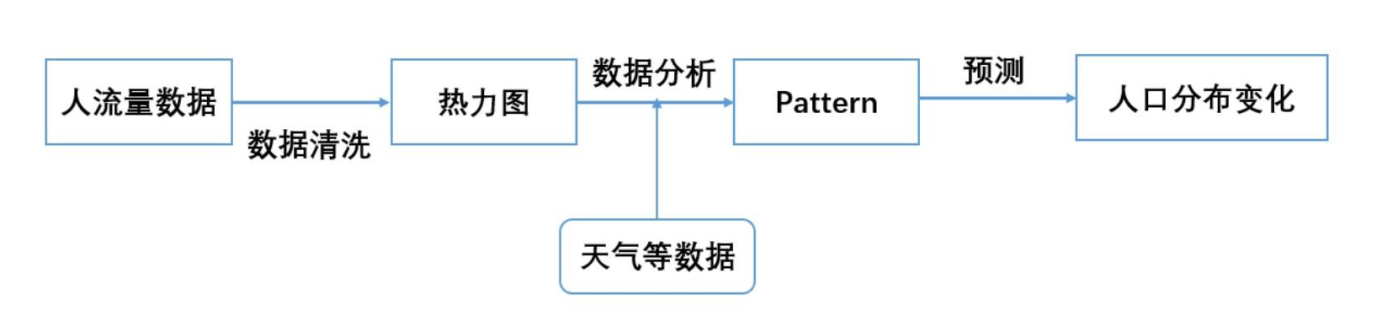
\includegraphics[width=0.8\textwidth]{pattern.png}
\caption{项目分析思路}
\label{fig:pattern}
\end{figure}
\subsection{代码架构}
分析代码见 \\ \url{https://github.com/BigDataSystemTHU2018/Project-Unicom/tree/master/Code}
问题的主要模块分析如下:
\begin{itemize}
	\item 问题分析阶段
		\begin{itemize}
			\item 问题描述:用过去三个月的信令数据预测未来一个周的人口分布,即已知过去三个月的数据,(尽可能)预测未来一周的数据
			\item 问题性质:回归
			\item 评判指标:预测出的结果尽可能的准确,即预测值与实际误差尽可能小。
		\end{itemize}
	\item 设计阶段——设计出一个回归系统,输入为过去三个月的数据,输出为已有数据的分析结果和预测结果。系统包含以下几个模块:
		\begin{itemize}
			\item 预处理模块:
			输入为原始数据,输出为清洗后的数据。负责数据的清洗,缺失值补全,异常值噪声点的处理等
			\item 预分析模块:
			负责从已有数据中提取挖掘先验知识,数据初步分析,可视化等。
			\item 回归前处理模块:
			将数据归一化等。
			\item 回归器模块:
			用于预测
			\item 回归后处理模块:
			包括可视化,对预测数据分析,生成报告等等。
		\end{itemize}
	\item 编码阶段——技术路线:
		\begin{itemize}
			\item 平台:tensorflow,sklearn
			\item 算法:聚类(K-means),降维(PCA/NMF),回归(MLP/ResNet)
			\item 可视化:matlab, matplotlib(seaborn)
		\end{itemize}
\end{itemize}
\subsubsection*{回归器结构}
回归系统的回归器分为4个部分,分别是:数据处理、Resnet搭建、网络训练、模型预测,其代码见\\ \url{https://github.com/BigDataSystemTHU2018/Project-Unicom/tree/master/Code/Processor/ResNet})\\ 模块的主要功能为:
\begin{enumerate}
	\item 从本地目录获取所有清洗好的数据,将数据按照Resnet的要求加载到内存。
	\item 对数据自动分为训练数据和预测数据,其中训练数据喂入Resnet进行模型训练。
	\item 对训练好的模型进行预测结果的输出。
	\item 支持断点续训,训练过程中模型会每10轮保存一次,可以自由跳转到已经保存好的模型进行继续训练或者模型输出。
	\item 支持迁移学习。即利用已经训练好的模型训练新的场景,提高训练的效率和降低对样本数量的需求。
	\item getdataTHU.py: 搜索当前目录下所有.csv,.txt文件,以这些文件作为所需的数据。请将待训练的数据放入当前目录。
	\item ResnetTHU.py: 定义网路结构,可以根据需要改变卷积核大小(CONV\_SIZE)和激活函数。
	\item trainTHU.py: 训练模块,也为反向传播模块,根据需要可以改变图片大小
	IMAGE\_WIDTH,IMAGE\_HIGHT,改变通道数NUM\_CHANNELS1,\\
	NUM\_CHANNELS2,NUM\_CHANNELS3,同时BATCH\_SIZE2,BATCH\_SIZE3\\,BATCH\_SIZE4也要相应的改变来保持一致(现为取最近3小时,一天前的4小时,一周前的2小时)。
	\item predictTHU.py: 预测模块,需要设置预测天数(现为7天)。
\end{enumerate}
模型网络的基本逻辑架构如图(\ref{fig:B1})所示:
\begin{figure}[ht]
\centering
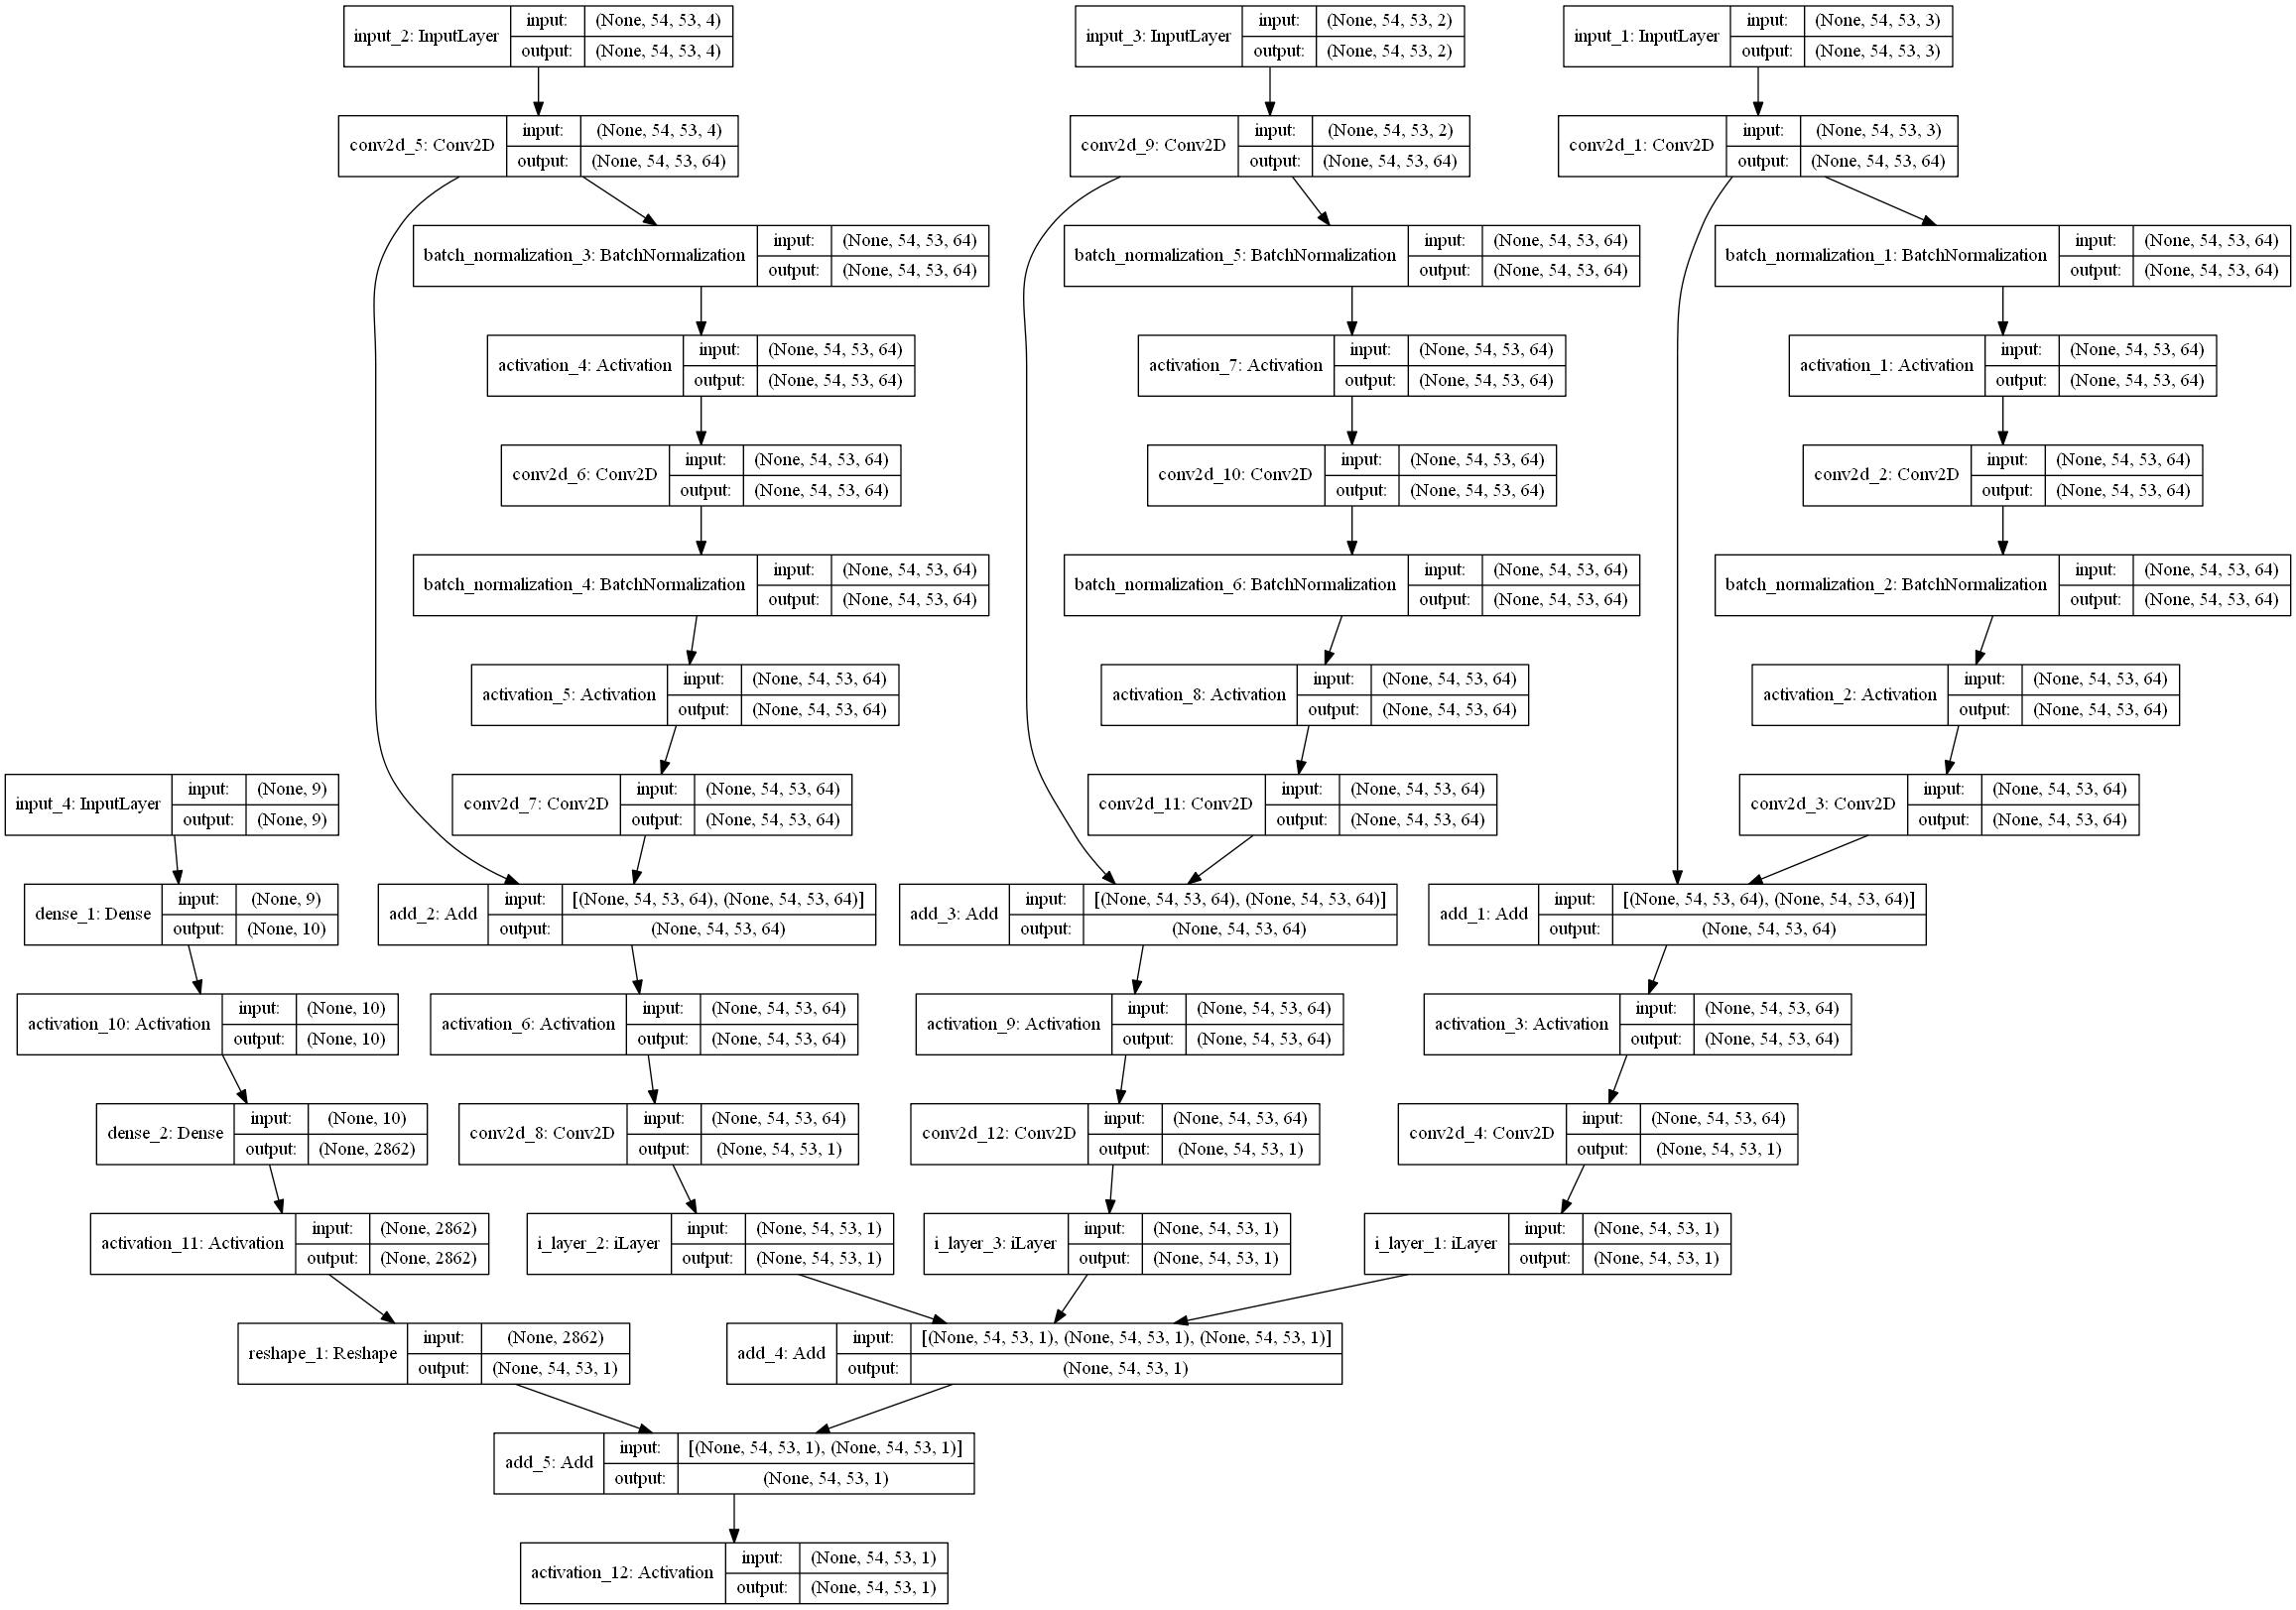
\includegraphics[width=0.8\textwidth]{B2.png}
\caption{残差网络构型}
\label{fig:B1}
\end{figure}
